\section{Auswertung}
\label{sec:Auswertung}
In diesem Abschnitt werden nun die Messungen der verschiedenen Würfel ausgewertet und die linearen Abschwächungskoeffizienten bestimmt.
Alle erstellten Grafiken und Rechnungen werden mit Python \cite{python} durchgeführt. Um zu Gewährleisten, dass der statistische Poissonfehler unterhalb von 3\% liegt, wird folgende Formel benutzt:
\begin{equation}
  \dfrac{1}{\sqrt{N}} < \num{0,03}
\end{equation}
Daraus folgt, dass ab einer Countzahl $N>1112$ der statistische Fehler unterhalb von 3\% liegt.
\subsection{Spektrum mit leerem Würfel}
Zunächst wird eine Messung durchgeführt, in der sich ein leerer Aluminiumwürfel im Strahlengang befindet. Dabei ergibt sich das Spektrum in Abbildung (\ref{fig:alu_leer}).
\begin{figure}
	\centering
	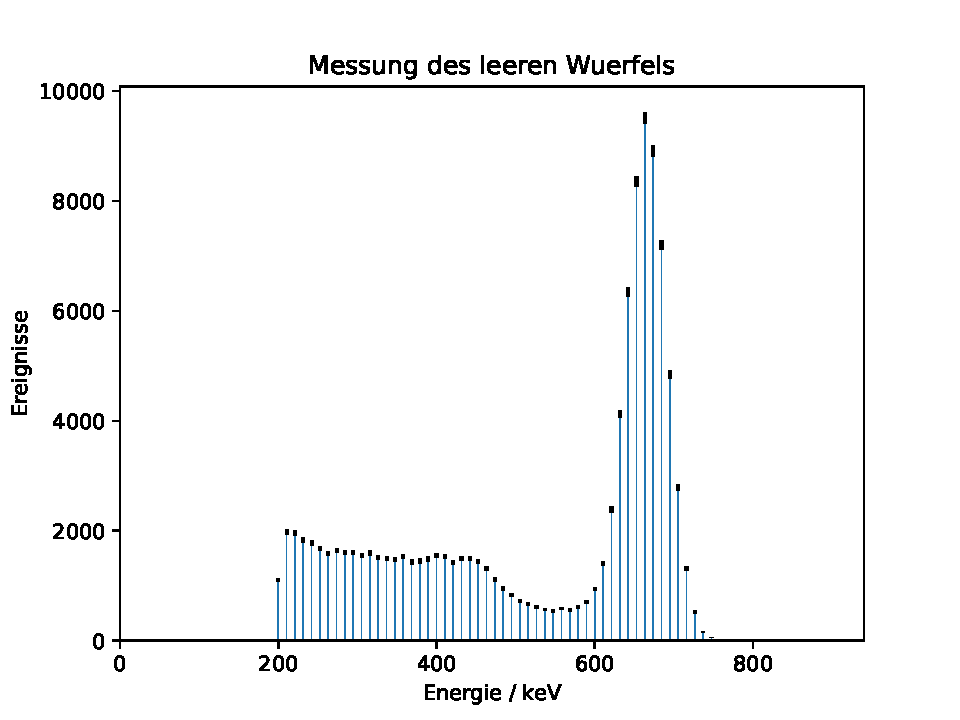
\includegraphics[scale=0.7]{fig/Alu_leer.pdf}
	\caption{Aufgenommenes Spektrum mit der Alumminiumhülle.}
	\label{fig:alu_leer}
\end{figure}
\FloatBarrier
\noindent Ebenfalls wird aus dieser Messung die für die anderen Würfel verwendete Zählrate $I_\mathrm{0}$ bestimmt. In $t_\mathrm{mess}=\SI{300}{\second}$ werden dabei $N=49361$ Impulse aufgezeichnet. Daraus ergibt sich die Zählrate zu $I_\mathrm{0}=\num{164.5(7)}\dfrac{\mathrm{Counts}}{\si{\second}}$.
\subsection{Aluminiumwürfel und Bleiwürfel}
Für die Würfel aus einheitlichem Material werden vier verschiedene Weglängen gemessen, da mehr Projektionen nicht benötigt werden. Da der Würfel nur aus einem Material besteht, können die Werte der verschiedenen Projektionen für $\vec{I}$ für gleiche Weglängen verwendet werden. \\
Weiter kann die Geometriematrix $A$ aufgrund des einheitlichen Materials durch einen Vektor dargestellt werden, in dem die einzelnen Komponenten für gleiche Wegstrecken aufsummiert werden.
Damit folgt für die Würfel:
\begin{equation}
  A=
  \begin{pmatrix}
    3 \\
    3\sqrt{2} \\
    2\sqrt{2} \\
    \sqrt{2}
  \end{pmatrix} \, .
\end{equation}
\FloatBarrier
\noindent Für den Aluminiumwürfel ergibt sich $\vec{I}_\mathrm{Alu}$ und $\vec{\tilde{I}_\mathrm{Alu}}$ zu:
\begin{equation}
	\vec{I}_\mathrm{Alu}=
	\begin{pmatrix}
		140,9\,\pm\,0,7 \\
		136,4\,\pm\,0,7 \\
		143,8\,\pm\,0,7 \\
    152,8\,\pm\,0,7
	\end{pmatrix}
	\frac{\mathrm{Counts}}{\si{\second}}\quad
	\vec{\tilde{I}_\mathrm{Alu}}=
	\begin{pmatrix}
		0,16\,\pm\,0,08 \\
		0,19\,\pm\,0,08 \\
		0,14\,\pm\,0,08 \\
    0,07\,\pm\,0,08
	\end{pmatrix}
	\label{eqn:w2}
\end{equation}
\FloatBarrier
\noindent Für den Bleiwürfel ergibt sich $\vec{I}_\mathrm{Blei}$ und $\vec{\tilde{I}_\mathrm{Blei}}$ zu:
\begin{equation}
	\vec{I}_\mathrm{Blei}=
	\begin{pmatrix}
		5,1\,\pm\,0,1 \\
		2,21\,\pm\,0,09 \\
		8,9\,\pm\,0,2 \\
    49,7\,\pm\,0,4
	\end{pmatrix}
	\frac{\mathrm{Counts}}{\si{\second}}\quad
	\vec{\tilde{I}_\mathrm{Blei}}=
	\begin{pmatrix}
		3,5\,\pm\,0,4 \\
		4,3\,\pm\,0,7 \\
		2,9\,\pm\,0,3 \\
    1,2\,\pm\,0,1
	\end{pmatrix}
	\label{eqn:w3}
\end{equation}
\FloatBarrier
\noindent Die Methode der kleinsten Quadrate liefert zusammen mit Gleichung (\ref{eqn:mu}) die Absorptionskoeffizienten und deren Unsicherheiten für die jeweiligen Materialien.
In Tabelle \ref{tab:tabalu} sind die Ergebnisse für beide Würfel angegeben.
\begin{table}
  \centering
  \caption{Ergebnisse für die Bestimmung der Absorptionskoeffizienten von den Würfeln 2 und 3.}
  \label{tab:tabalu}
  \begin{tabular}{c c c}
    \toprule
		$\mathrm{Würfelnummer}$ & $\mu \: [\si{1\per\centi\meter}]$ & $\mathrm{Material}$ \\
    \midrule
		$\num{2}$ & $\num{0,04(1)}$ & $\mathrm{Aluminium}$\\
		$\num{3}$ & $\num{0,98(6)}$ & $\mathrm{Blei}$ \\
    \bottomrule
  \end{tabular}
\end{table}
\FloatBarrier
\subsection{Würfel aus diversen Materialien}
\noindent In diesem Teil wird nun der Würfel, der aus verschiedenen Materialien zusammengesetzt ist untersucht. Im Gegensatz zu den Würfeln aus einheitlichem Material werden hier zwölf Projektionen
zur Vermessung verwendet. Damit ergibt sich für die Geometriematrix $A_\mathrm{2}$:
\begin{equation}
  \label{eqn:geomat}
	A_\mathrm{2}=
	\begin{pmatrix}
    1 & 1 & 1 & 0 & 0 & 0 & 0 & 0 & 0 \\
    0 & 0 & 0 & 1 & 1 & 1 & 0 & 0 & 0 \\
    0 & 0 & 0 & 0 & 0 & 0 & 1 & 1 & 1 \\
    1 & 0 & 0 & 1 & 0 & 0 & 1 & 0 & 0 \\
    0 & 1 & 0 & 0 & 1 & 0 & 0 & 1 & 0 \\
    0 & 0 & 1 & 0 & 0 & 1 & 0 & 0 & 1 \\
    0 & \sqrt{2} & 0 & \sqrt{2} & 0 & 0 & 0 & 0 & 0 \\
    0 & 0 & \sqrt{2} & 0 & \sqrt{2} & 0 & \sqrt{2} & 0 & 0 \\
    0 & 0 & 0 & 0 & 0 & \sqrt{2} & 0 & \sqrt{2} & 0 \\
    0 & \sqrt{2} & 0 & 0 & 0 & \sqrt{2} & 0 & 0 & 0 \\
    \sqrt{2} & 0 & 0 & 0 & \sqrt{2} & 0 & 0 & 0 & \sqrt{2} \\
    0 & 0 & 0 & \sqrt{2} & 0 & 0 & 0 & \sqrt{2} & 0 \\
	\end{pmatrix}
\end{equation}
\FloatBarrier
\noindent Die Spalten der Matrix geben dabei jeweils die Position des Würfels an (siehe Abbildung (\ref{fig:aufbau})).
Weiter gilt für den Projektionsvektor $\vec{I}_\mathrm{div}$ und sowie für $\vec{\tilde{I}}_\mathrm{div}$:
\begin{equation}
	\vec{I}_\mathrm{div}=
	\begin{pmatrix}
		49,3\,\pm\,0,4 \\
		46,5\,\pm\,0,4 \\
		44,4\,\pm\,0,4\\
		115,7\,\pm\,0,6 \\
		5,9\,\pm\,0,1 \\
    128,3\,\pm\,0,7 \\
		32,8\,\pm\,0,3 \\
		27,6\,\pm\,0,3 \\
		39,7\,\pm\,0,4 \\
		40,3\,\pm\,0,4 \\
		28,8\,\pm\,0,7 \\
    49,8\,\pm\,0,4
	\end{pmatrix}
	\frac{\mathrm{Counts}}{\si{\second}}\quad
	\vec{\tilde{I}}_\mathrm{div}=
	\begin{pmatrix}
    1,2\,\pm\,0,1 \\
		1,3\,\pm\,0,1 \\
		1,3\,\pm\,0,2 \\
		0,35\,\pm\,0,09 \\
		3,3\,\pm\,0,4 \\
    0,25\,\pm\,0,09 \\
		1,6\,\pm\,0,2 \\
		1,8\,\pm\,0,2 \\
		1,4\,\pm\,0,2 \\
		1,4\,\pm\,0,2 \\
		1,7\,\pm\,0,2 \\
    1,2\,\pm\,0,1
	\end{pmatrix}
	\label{eqn:w5}
\end{equation}
\FloatBarrier
\noindent Die Methode der kleinsten Quadrate liefert für die Absorptionskoeffizienten die Ergebnisse in Tabelle \ref{tab:tabdiv}:
\begin{table}
  \centering
  \caption{Ergebnisse für die Bestimmung der Absorptionskoeffizienten des unbekannten Würfel.}
  \label{tab:tabdiv}
  \begin{tabular}{c c c}
    \toprule
		$\mathrm{Position ~ des ~ Würfel}$ & $\mu \: [\si{1\per\centi\meter}]$ & $\mathrm{Vermutetes ~ Material}$ \\
    \midrule
    $\num{1}$ & $\num{0,08(9)}$ & $\mathrm{Delrin}$ \\
		$\num{2}$ & $\num{1,04(8)}$ & $\mathrm{Blei}$ \\
		$\num{3}$ & $\num{0,03(9)}$ & $\mathrm{Delrin}$ \\
    $\num{4}$ & $\num{0,04(7)}$ & $\mathrm{Delrin}$ \\
    $\num{5}$ & $\num{1,06(8)}$ & $\mathrm{Blei}$ \\
    $\num{6}$ & $\num{0,07(7)}$ & $\mathrm{Delrin}$ \\
    $\num{7}$ & $\num{0,22(9)}$ & $\mathrm{Aluminium}$ \\
    $\num{8}$ & $\num{0,88(7)}$ & $\mathrm{Blei}$ \\
    $\num{9}$ & $\num{0,14(9)}$ & $\mathrm{Delrin}$ \\
    \bottomrule
  \end{tabular}
\end{table}
\FloatBarrier
